\chapter{Raw Materials}
\label{chap:raw}

The prototypical memristor was based on a titanium dioxide thin film sandwiched between metallic electrodes \cite{Williams2008}, and many other devices have been manufactured by following the same recipe \cite{Szot2011,Kwon2010,Jeong2012,Pan2014}. Experimental data shows that oxygen-deficient phases of TiO$_2$ are formed inside the oxide layer of these devices \cite{Kwon2010,HwanKim2011}. For this reason, we start our bottom-up study of the devices by investigating the electronic structure of the non-stoichiometric compounds known as the Magnéli phases (Ti$_n$O$_{2n-1}$, $n = 4, 5$) as well as the Ti$_2$O$_3$-corundum structure and the $\alpha-$, $\beta-$, and $\gamma-$ phases of Ti$_3$O$_5$. 

\begin{center}
 \begin{table}[h!]
  \centering
   \caption{\label{tab:symm} International and Schoenflies notations for the space groups of TiO$_2$-rutile, and Ti${}_n$O${}_{2n-1}$, ($2 \leq n \leq 5$) \cite{Belsky2002,Aroyo2006}.}
   \begin{tabular}{p{0.2\columnwidth}p{0.3\columnwidth}p{0.2\columnwidth}} 
   \hhline{===}
                              & \multicolumn{2}{c}{Space Group}    \\
                              & International (\#) &  Schoenflies  \\
    \hline
    TiO$_2$-rutile			  & $P4_2/mnm$ (136)   & $D_{4h}$      \\
    Ti${}_2$O${}_3$           & $R\bar{3}c$ (167)  & $D_{3d}$      \\
    $\alpha$-Ti${}_3$O${}_5$  & $Cmcm$ (63)        & $D_{2h}$      \\
    $\beta$-Ti${}_3$O${}_5$   & $C2/m$ (12)        & $C_{2h}$      \\
    $\gamma$-Ti${}_3$O${}_5$  & $C2/c$ (15)        & $C_{2h}$      \\
    Ti${}_4$O${}_7$           & $P\bar{1}$ (2)     & $C_i$         \\
    Ti${}_5$O${}_9$           & $P1$ (1)           & $C_1$  \\ 
    \hhline{===}
   \end{tabular}
 \end{table}
\end{center}

Table \ref{tab:symm} presents the space groups of the systems studied at this stage. The structures present larger unit cells as $n$ in Ti$_n$O$_{2n-1}$ becomes larger. In fact, the larger the value of $n$, the closer to stoichiometric TiO$_2$: for $n > 37$ the structure is rutile with point defects or Wadsley defects \cite{Szot2011}. On the other hand, for smaller values of $n$, the formation of new structures was reported by Andersson and Magnéli \cite{Andersson1957}.

For all systems the equilibrium lattice constants and ion positions were obtained via DFT calculations. Two approximations were used for the exchange-correlation functional: GGA approximation via PBESol functional and screened hybrid as implemented in HSE. The relaxation output data is presented in the table \ref{tab:struct-relax-prb}. The error in comparison with experimental data from X-ray diffraction spectra was considered small, being the highest deviation for $\alpha$-Ti$_3$O$_5$ close to 6\% with respect to unit cell volume. Further details of the parameters used in all calculations can be found in appendix \ref{sec:app-calc}.
 \begin{table*}[ht!]
  \centering
  \caption{\label{tab:struct-relax-prb} Experimental and theoretical values of lattice parameters for the Ti${}_2$O${}_3$, $\alpha-$, $\beta-$ and $\gamma$-Ti${}_3$O${}_5$, Ti${}_4$O${}_7$, and Ti${}_5$O${}_9$ structures. Mean Absolute Relative Error for unit cell volume is also presented in parenthesis. Values presented are those of the primitive cells.}
   \begin{tabular}{*{2}{p{0.012\textwidth}} p{0.14\textwidth} *{3}{p{0.06\textwidth}} *{3}{p{0.07\textwidth}} *{1}{p{0.18\textwidth}}} 
  \hhline{==========}
       &               &                          & $a$(\AA) & $b$(\AA) & $c$(\AA) & $\alpha$(${}^{\mathrm{o}}$) & $\beta$(${}^{\mathrm{o}}$) & $\gamma$(${}^{\mathrm{o}}$) & $\Omega$ (\AA${}^3$) \\
  \hhline{==========}
  &  &    Exp\cite{Robinson1974,Abrahams1963} & 5.433 & -      & -        & 56.57  & -      & -                         & 160.37               \\
  &  &    PBESol                              & 5.471   & -      & -        & 54.89  & -      & -                         & 163.80 (2.14\%)      \\
  \multicolumn{2}{c}{\multirow{-3}{*}{\begin{sideways}Ti${}_2$O${}_3$\end{sideways}}} &  HSE           & 5.370  & -      & -        & 57.62   & -      & -               & 154.87 (3.43\%)       \\
             \hhline{==========}
       &               & Exp\cite{Rusakov2002}    & 3.747    & 5.090    & 9.715    & 90.00                       & 90.00                      & 68.40                       & 172.27 \\
       &      $\alpha$ & PBESol                   & 3.760    & 5.237    & 9.937    & 90.00                       & 90.00                      & 68.96                       & 182.60 (6.00\%) \\
       &               & HSE                      & 3.682    & 5.258    & 9.978    & 90.00                       & 90.00                      & 69.50                       & 180.94 (5.03\%) \\
             \cline{2-10}
       &               & Exp\cite{Asbrink1959} & 3.802    & 5.233    & 9.442    & 91.79                       & 90.00                      & 111.30                      & 174.94 \\
       &      $\beta$  & PBESol                   & 3.834    & 5.195    & 9.215    & 90.87                       & 90.00                      & 111.65                      & 170.60 (2.48\%) \\
       &               & HSE                      & 3.791    & 5.196    & 9.173    & 90.76                       & 90.00                      & 111.40                      & 168.23 (3.61\%) \\
             \cline{2-10}
      &                & Exp\cite{Hong1982}    & 5.075    & 5.658    & 7.181    & 109.58                      & 90.00                      & 116.64                      & 170.85 \\
     &        $\gamma$ & PBESol                   & 4.997    & 5.627    & 7.180    & 109.81                      & 90.00                      & 116.36                      & 167.45 (1.99\%) \\
   \multirow{-9}{*}{\begin{sideways}Ti${}_3$O${}_5$\end{sideways}} &                  & HSE                      & 5.076    & 5.664    & 7.069    & 109.36                      & 90.00                      & 116.62                      & 168.76 (1.22\%) \\
  \hhline{==========}
 &  &   Exp\cite{LePage1984} & 5.626    & 6.892    & 7.202    & 63.71                       & 109.68                     & 105.24                      & 233.60              \\
 &  &  PBESol               & 5.569    & 6.868    & 7.092    & 64.22                       & 109.72                     & 104.91                      & 229.12 (1.92\%)            \\
 \multicolumn{2}{c}{\multirow{-3}{*}{\begin{sideways}Ti${}_4$O${}_7$\end{sideways}}}  &  HSE                  & 5.618    & 6.898    & 7.076    & 63.77                       & 108.77                     & 104.23                      & 231.09 (1.07\%) \\
  \hhline{==========}
 &  &    Exp\cite{Andersson1960} & 5.569    & 7.120    & 8.865    & 97.55                       & 112.34                     & 108.50                      & 295.33              \\
 &  &   PBESol                  & 5.558    & 7.110    & 8.846    & 97.75                       & 112.51                     & 108.61                      & 292.54 (0.94\%)             \\
 \multicolumn{2}{c}{\multirow{-3}{*}{\begin{sideways}Ti${}_5$O${}_9$\end{sideways}}} &   HSE                     & 5.550    & 7.040    & 8.763    & 96.96                       & 112.35                     & 108.09                      & 289.68 (1.91\%) \\
  \hhline{==========}
   \end{tabular}
 \end{table*}

\section{TiO$_2$-rutile}
\label{sec:tio2}

Titanium dioxide (TiO$_2$) is the stoichiometric\footnote{The use of the term \textit{stoichiometric} in this thesis is justified by the same practice in the literature on the TiO phases. The stoichiometric compound is most of the time TiO$_2$, due to the fact that the Ti atom is in the $+4$ oxidation state with the 3s$^2$3p$^6$ configuration (3d and 4s are empty) and oxygen assumes the $-2$ state.} compound of the TiO family. Its naturally occurring structures are the rutile, anatase and brookite structures. While the first is the most stable one, anatase is metastable and brookite is a high-pressure phase \cite{Dachille1968}. Due to its low cost and high catalytic activity, TiO$_2$ is employed in a variety of applications, such as water-splitting for energy harvesting \cite{Scanlon2013}. TiO$_2$-rutile is a well known wide-bandgap (experimental value $E_g \approx 3.1$ eV \cite{Amtout1995}) semiconductor. 

\begin{figure}[!ht]
 \centering
  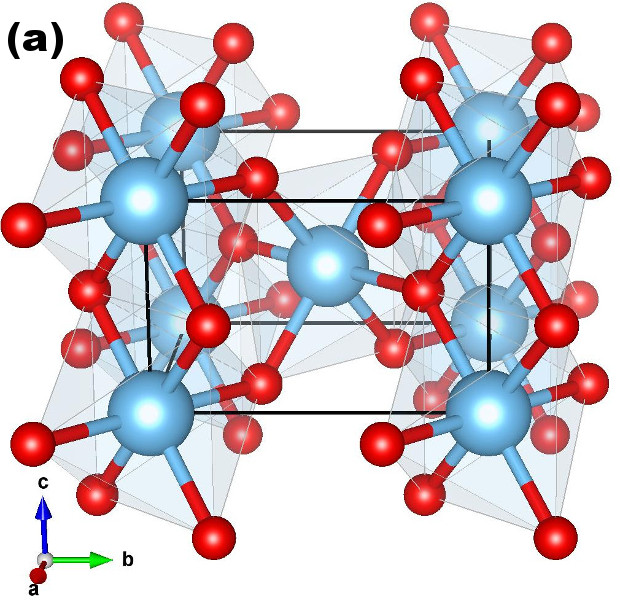
\includegraphics[height=5cm]{img/tio2-rutile.jpg}
  \qquad
  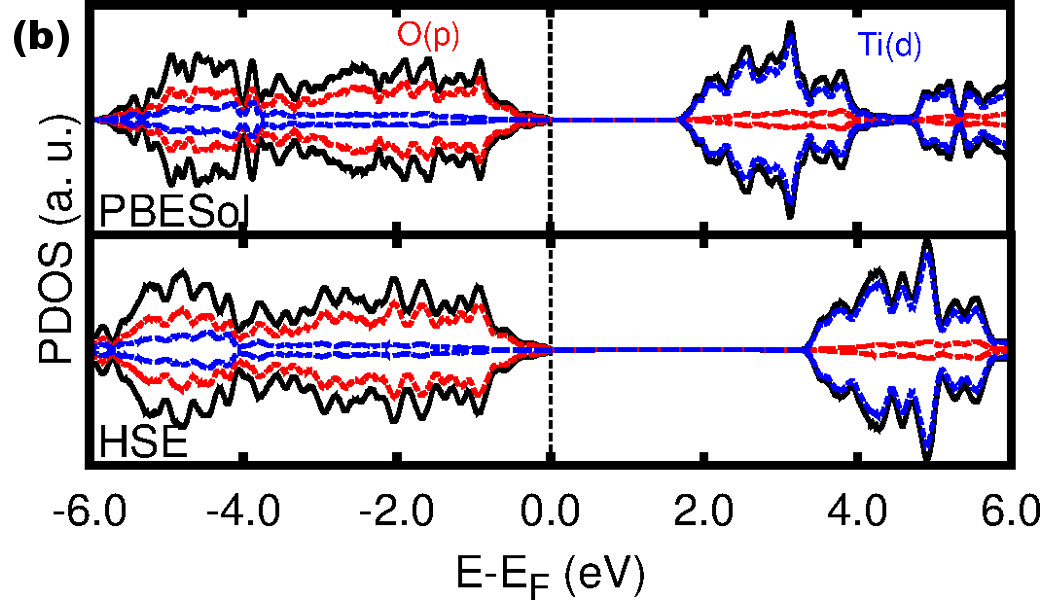
\includegraphics[height=5cm]{img/dos-tio2-rutile.jpg}
  \caption{(a) TiO$_2$-rutile structure. Blue spheres are Ti atoms and red spheres are O atoms. TiO$_6$ octahedra are featured by the transparent blue polyhedra enclosing the Ti atoms. (b) PDOS of TiO$_2$-rutile obtained either by PBESol (upper panel) and HSE (lower panel) functionals. The two spin components are depicted by positive and negative values along the vertical axis, and the vertical dashed line features the valence band maximum (VBM). The contribution from Ti(d) to CB and O(p) to VB are depicted by the blue and red dashed lines respectively while total DOS is given by the black full line.} 
  \label{fig:tio2}
\end{figure}

Its structure is depicted in figure \ref{fig:tio2} (a) where one can see the corner-sharing arrangement between its TiO$_6$ octahedra. The projected density of states (PDOS) was obtained for this compound using both the PBESol and HSE functionals and are presented in figure \ref{fig:tio2} (b). From these graphs one can notice that while the valence band (VB) is composed mainly by O(p) orbital contribution, the conduction band (CB) is mainly of Ti(d) character. It is also noticeable that HSE delivers a bandgap energy much closer to the experimental value than PBESol. This bandgap underestimation is a well known deficiency of GGA functionals \cite{Perdew2001}.

\section{Ti$_2$O$_3$-corundum}
\label{sec:ti2o3}

TiO presents a large range of non-stoichiometric compounds, and the most oxygen-deficient one before titanium monoxide (TiO) is the corundum structure Ti$_2$O$_3$. This compound presents a rhombohedral structure with space group $R\bar{3}c$ where its basic units, the TiO$_6$ octahedra, are displaced in face-sharing pairs, as shown in figure \ref{fig:struct-ti2o3}.
\begin{figure}[!ht]
 \centering
  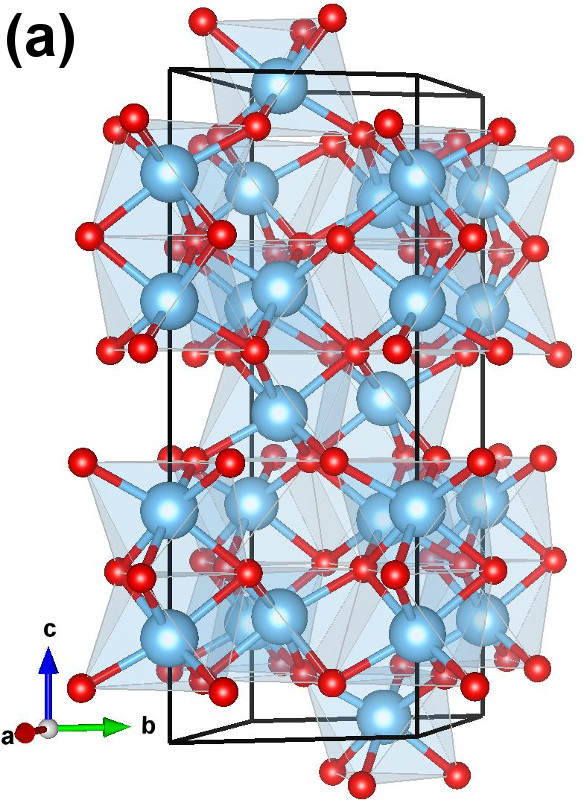
\includegraphics[height=7cm]{img/ti2o3-conv.jpg}
  \qquad
  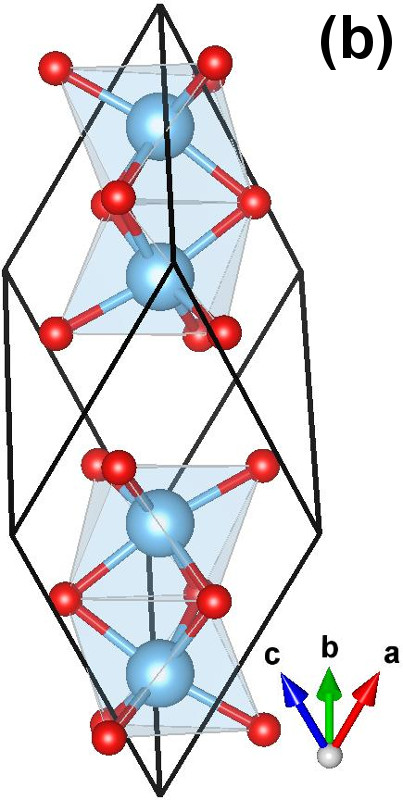
\includegraphics[height=7cm]{img/ti2o3-prim.jpg}
  \caption{Ti$_2$O$_3$ structures presented by the (a) conventional unit cell, and (b) primitive unit cell. Blue spheres are Ti atoms and red spheres are O atoms. TiO$_6$ octahedra are featured by the transparent blue polyhedra enclosing the Ti atoms.} 
  \label{fig:struct-ti2o3}
\end{figure}

As a first test of methodology, the band structure of the compound was obtained using the Local Density Approximation togheter with the Hubbard $U$ parameter (LDA$+U$), where the $U$ parameter was set to Ti(d) orbitals and its value was tuned in order to understand the impact in the final results. The same calculations were performed using the PBESol functional and the HSE functional for comparison. Results are presented in Figure \ref{fig:bands-ti2o3} where it is noticeable the effect of increasing $U$: two half-filled bands in $U = 0$ and PBESol calculations become splitted from the unoccupied bands above, thus revealing a semiconductor behavior for higher values of $U$ and for the hybrid HSE functional calculation\footnote{The $U$ parameter is usually employed in electronic structure calculations aiming to correct the DFT bandgap issue: the Local Density Approximation (LDA) and Generalized Gradient Approximation (GGA) are known to result in overestimated bandgaps. However, this bandgap correction is a consequence of a better localization of d or f electrons, due to an on-site Coulomb interaction (see appendix \ref{sec:app-dftu} and references therein for further details)}. This last result is in agreement with the experimental data, which states that this material is an insulator for low temperatures \cite{Uchida2008,Guo2012}.
\begin{figure}[!ht]
 \centering
  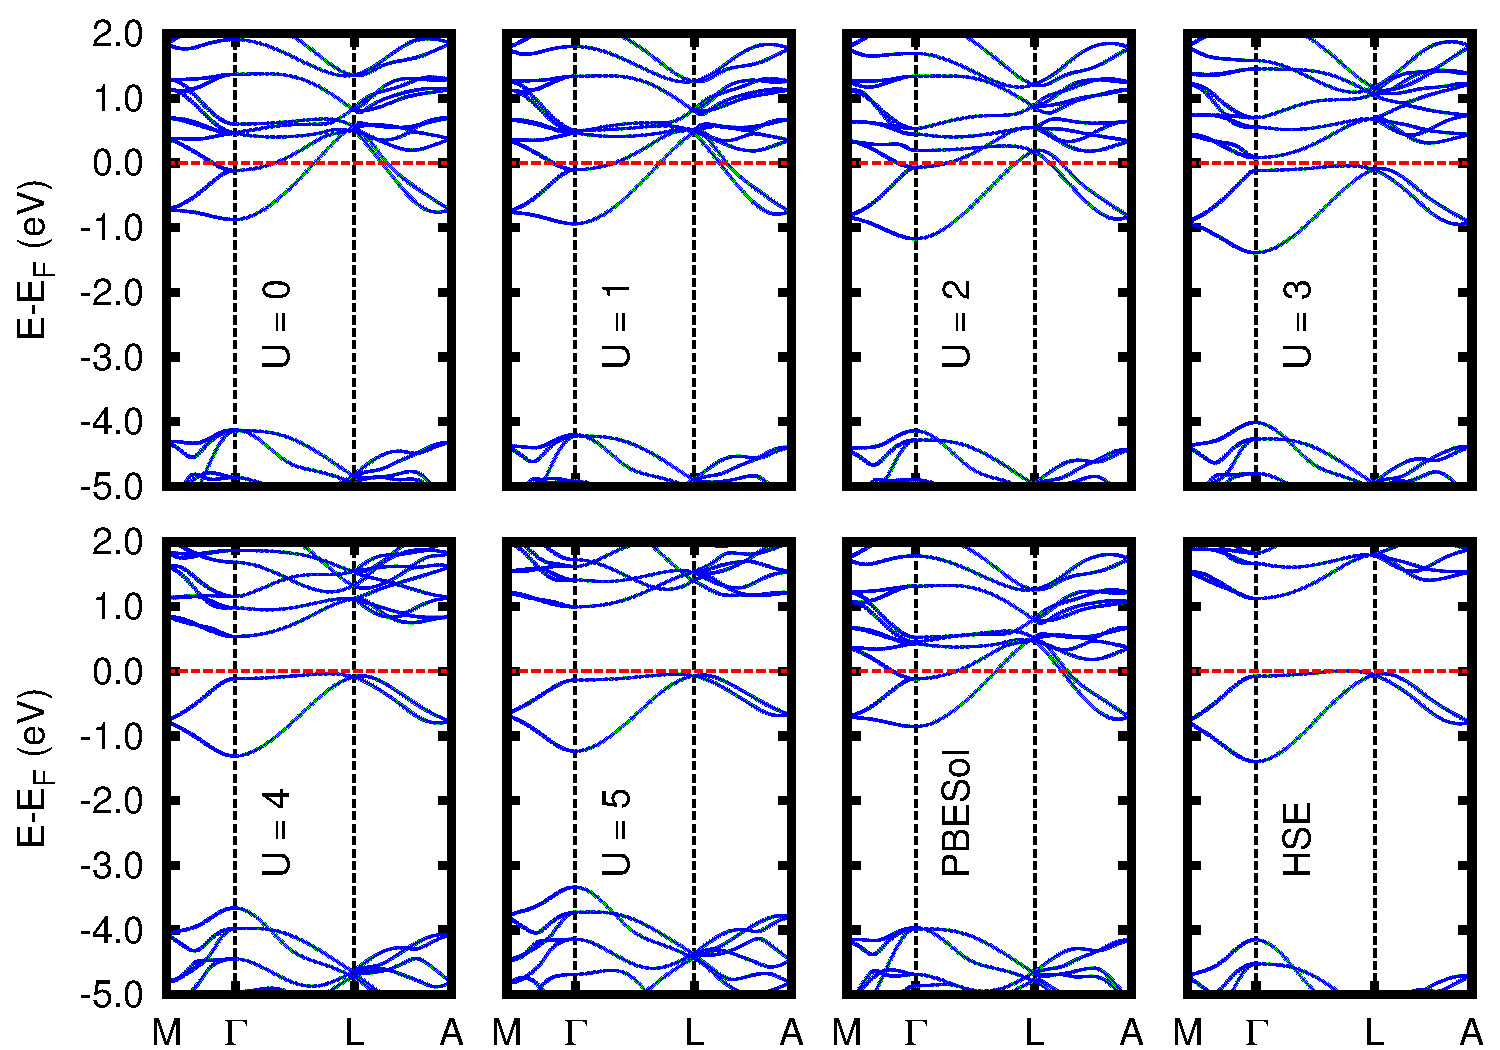
\includegraphics[width=0.95\textwidth]{img/ti2o3-bands.jpg}
  \caption{Band structure of Ti$_2$O$_3$ obtained using LDA+$U$ for increasing values of the Hubbard parameter $U$, ($0 \leq U \leq 5$) as well as PBESol and HSE functionals. The vertical red dashed line at zero energy is the Fermi energy. For $U \geq 3$ eV, as well as for the HSE calculation the system is a semiconductor, while in the other situations it is a metal.} 
  \label{fig:bands-ti2o3}
\end{figure}

 The PDOS was calculated using both PBESol, PBESol+$U$ ($U = 5$ eV) and HSE functionals and is presented in figure \ref{fig:dos-ti2o3-prb}. Once more the equivalence of the use of Hubbard $U$ and hybrid functional HSE is evident, and the incorrect description of a metal is provided solely by GGA functional PBESol. Another important information extracted form the PDOS is that the CB is mainly Ti(d), and when a bandgap is observed, the CB is also of the same character. In fact, this last occupied band can be regarded as an impurity band, very similar to the localized levels present in the TiO$_2$ bandgap when point defects are present \cite{Lee2012,Janotti2010}. The VB in this case can be identified as the levels laying around $-3$ eV for PBESol+U and $-4$ eV for HSE in figure \ref{fig:dos-ti2o3-prb}, mainly of O(p) character. In this picture, these systems have a large bandgap of $4-5$ eV and a filled intermediate band (IB) close to CBM, which could be an intrinsic $n$ dopant for the material.  
 
 \begin{center}
  \begin{figure}[ht!]
      \begin{center}
        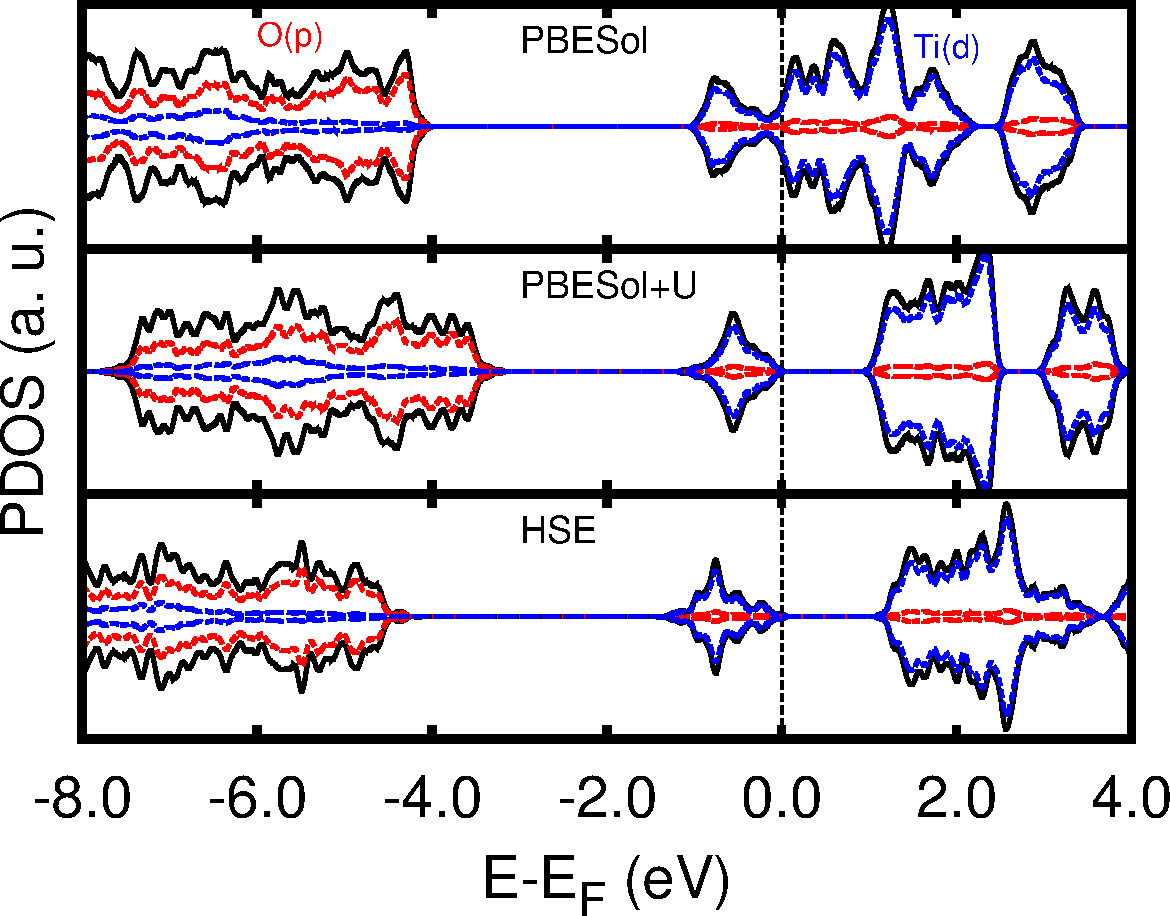
\includegraphics[width=0.6\textwidth]{img/dos-ti2o3-prb.jpg}
      \end{center}
      \caption{PDOS of Ti$_2$O$_3$ calculated by PBESol (upper panel), PBESol$+U$, where $U = 5$ eV (middle panel), and HSE (lower panel). The two spin components are depicted by positive and negative values along the vertical axis, and the vertical dashed line features the most energetic occupied level. The contribution from Ti(d) to CB and O(p) to VB are depicted by the blue and red dashed lines respectively while total DOS is given by the black full line.}.
      \label{fig:dos-ti2o3-prb} 
  \end{figure}
 \end{center}

The real-space projections of the IB (for PBESol the levels taken into account were the ones lower than $E_F$) are presented in figure \ref{fig:parchg-ti2o3-prb}. From these projections, it is evident that both the PBESol$+U$ and HSE calculations resulted in better descriptions of the Ti(d)-like levels, presenting the same hybridization. This was expected due to the fact that the introduction of the $U$ parameter leads to a stronger localization of these electrons arising from the on-site Coulomb interaction while the HSE functional introduces a part of the exact exchange, leading to a partial cancellation of the self-interaction problem of DFT \cite{Kim2009}. For a more detailed discussion please see appendices \ref{sec:app-dftu} and \ref{sec:app-hybrid}.
 \begin{center}
  \begin{figure}[ht!]
      \begin{center}
        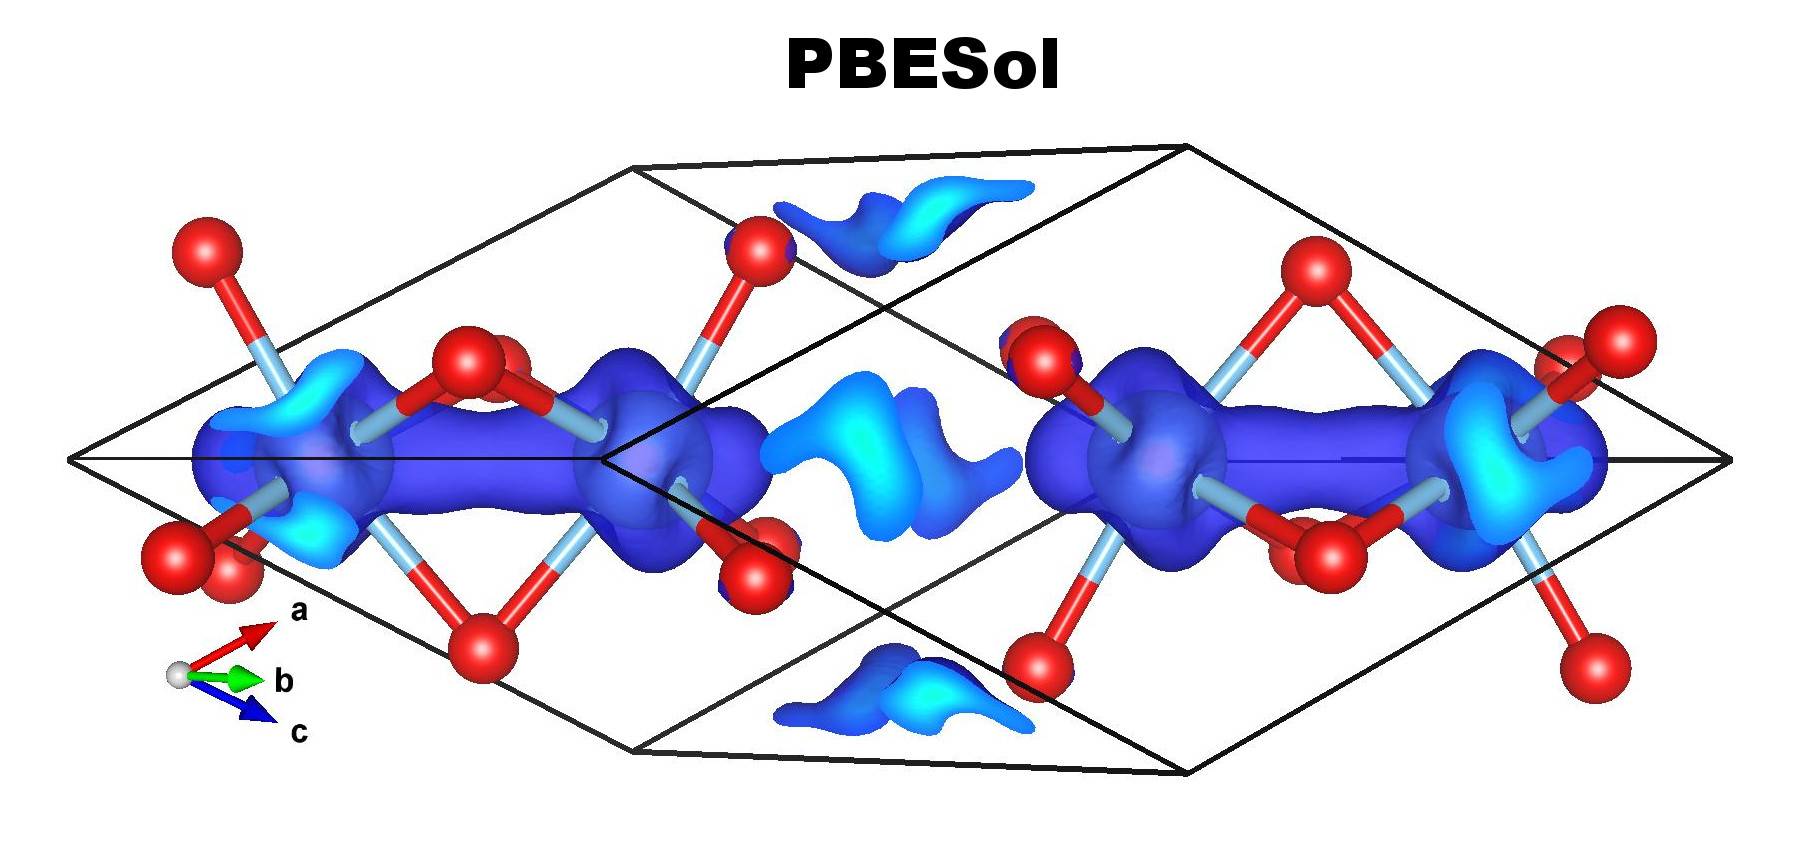
\includegraphics[width=0.3\textwidth]{img/ti2o3-parchg-pbesol+u-0.jpg}
        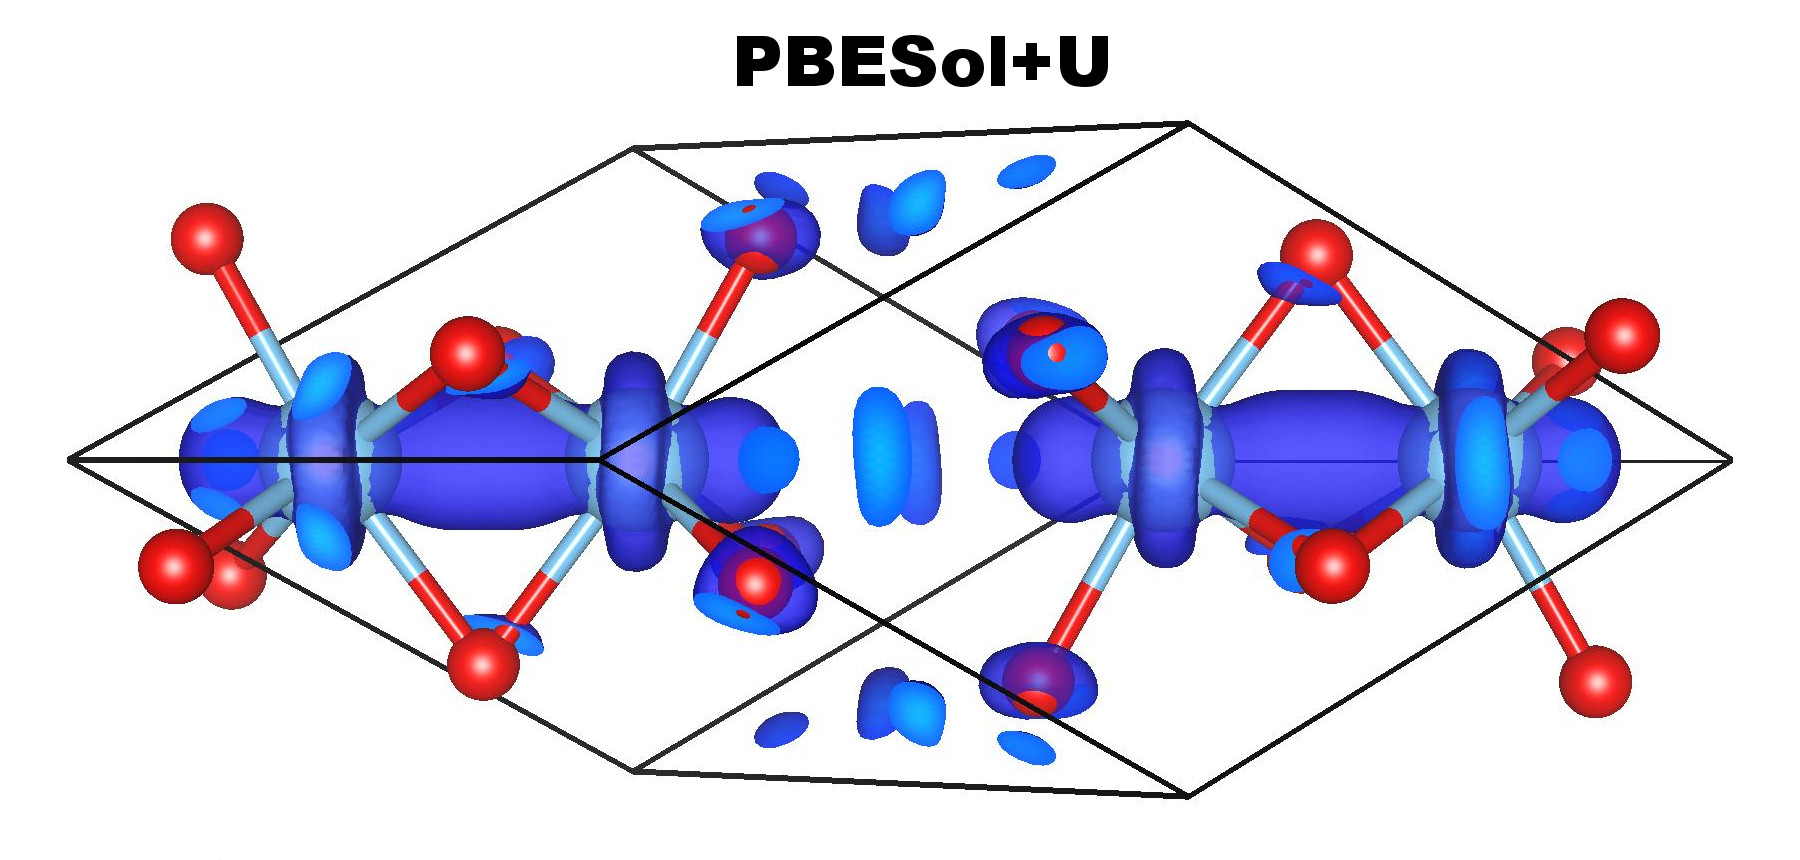
\includegraphics[width=0.3\textwidth]{img/ti2o3-parchg-pbesol+u-5.jpg}
        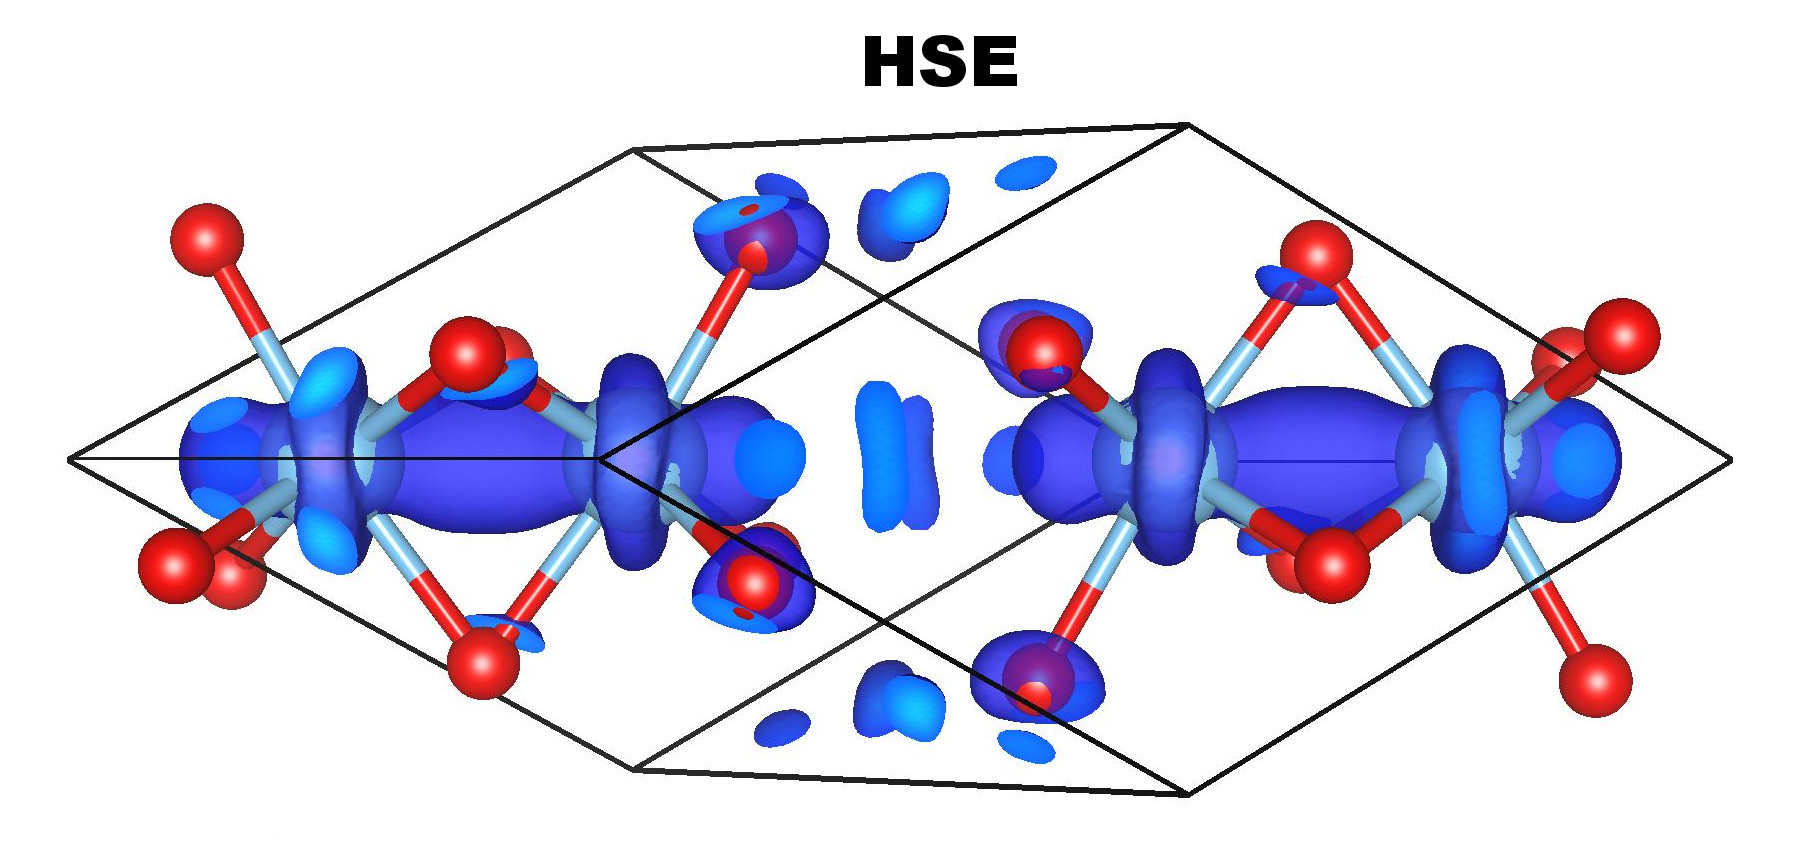
\includegraphics[width=0.3\textwidth]{img/ti2o3-parchg-hse.jpg} 
      \end{center}
      \caption{Real-space projection of the IB of Ti$_2$O$_3$ calculated by PBESol (left), PBESol$+U$, where $U = 5$ eV (middle), and HSE (right). The same isovalue of 1\% was used to plot the three bands.}.
      \label{fig:parchg-ti2o3-prb} 
  \end{figure}
\end{center}

\section{Ti$_3$O$_5$}

The crystal structure of Ti$_3$O$_5$ is not unique. A variety of phases were synthesized and characterized for this compound, thus, we chose to study the electronic structures of the three most common ones (presented in Figure \ref{fig:struct-ti3o5}): the $\alpha-$ (orthorhombic, anosovite-like, group $Cmcm$) \cite{Rusakov2002}, $\beta-$ (monoclinic, group C2/m) \cite{Asbrink1959,Grey1994}, and $\gamma-$Ti$_3$O$_5$ (monoclinic, $I2/c$) \cite{Hong1982}. A first-order phase transition at approximately $440-460$ K between $\alpha-$ and $\beta-$ phases was reported by Onoda \textit{et\ al.} \cite{Onoda1998} and another transition between $\beta-$ and $\gamma$-Ti$_3$O$_5$ close to $250$ K was reported by Hong and \AA sbrink \cite{Asbrink1959}. 
\begin{center}
  \begin{figure}[ht!]
      \begin{center}
        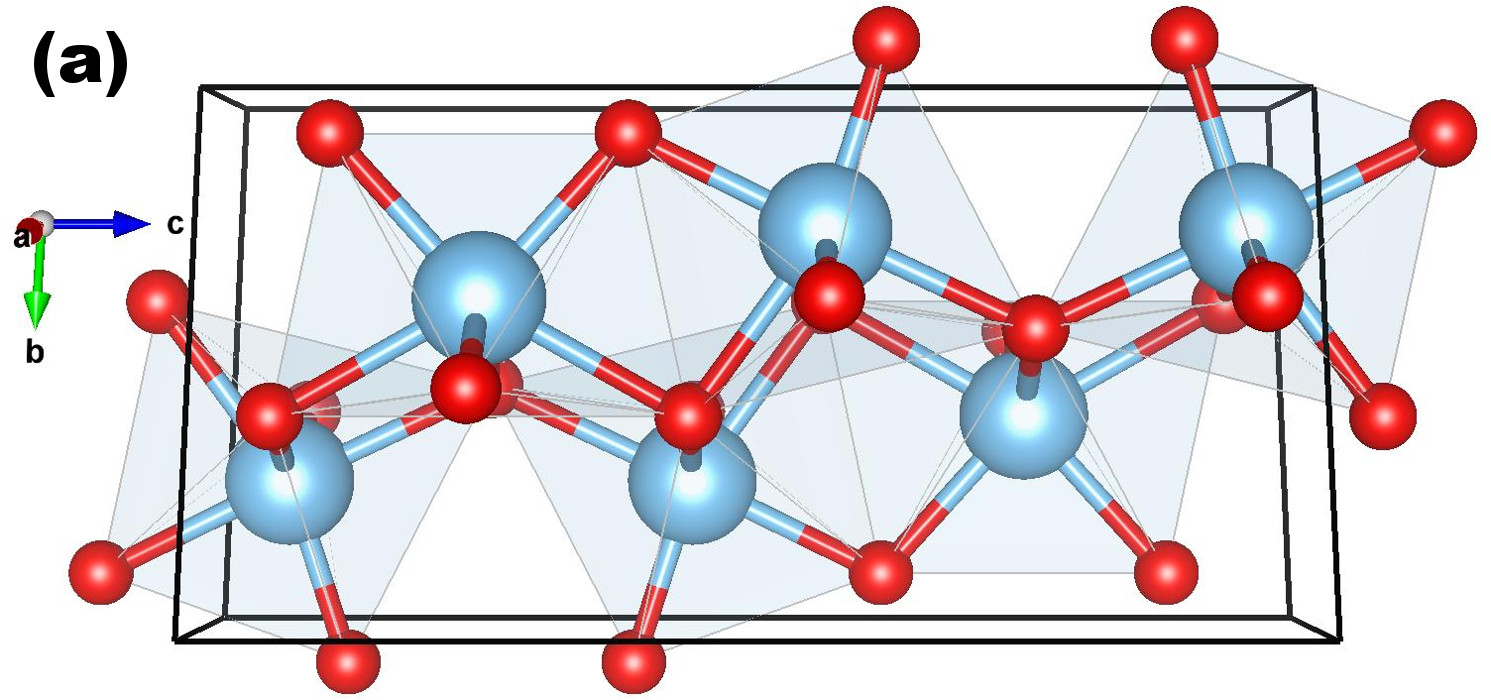
\includegraphics[height=2.5cm]{img/alpha-ti3o5.jpg}
        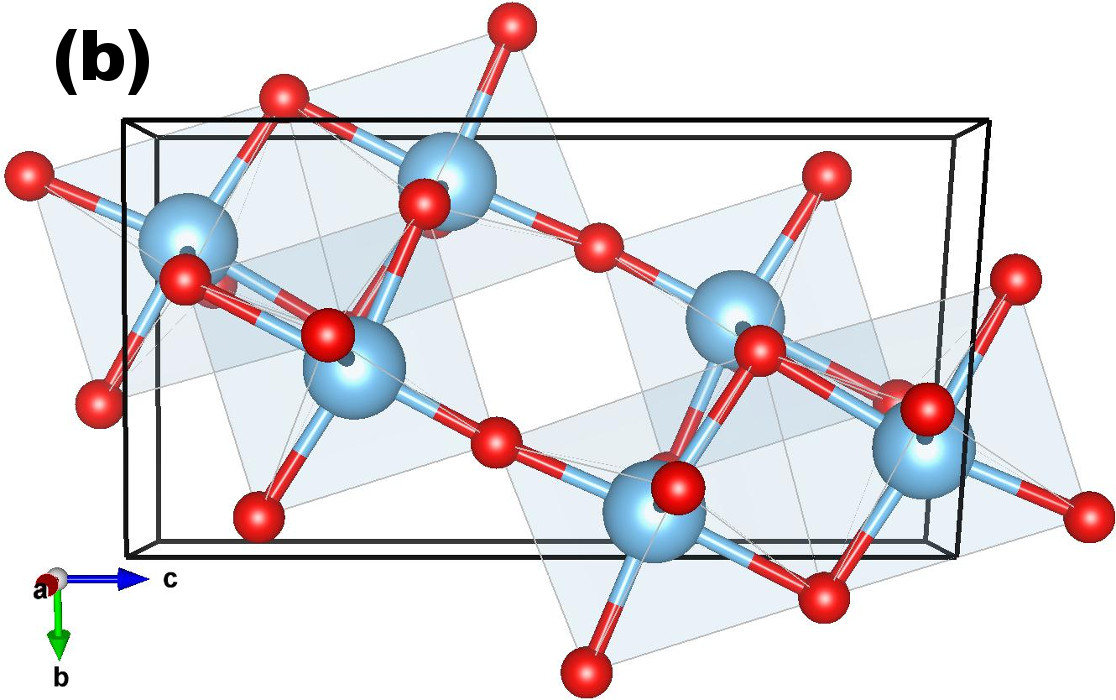
\includegraphics[height=2.5cm]{img/beta-ti3o5.jpg}
        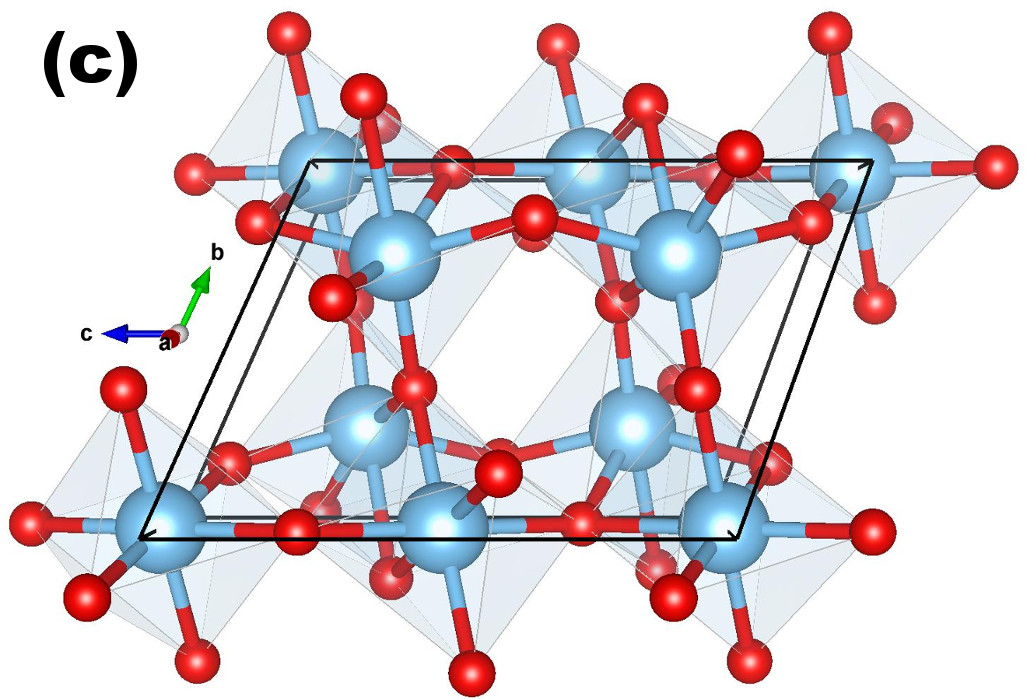
\includegraphics[height=2.5cm]{img/gamma-ti3o5.jpg} 
      \end{center}
      \caption{Crystalline structures of (a) $\alpha$-Ti$_3$O$_5$, (b) $\beta$-Ti$_3$O$_5$, and (c) $\gamma$-Ti$_3$O$_5$. Blue spheres are Ti atoms and red spheres O atoms. The TiO$_6$ octahedra are depicted in light blue.}
      \label{fig:struct-ti3o5} 
  \end{figure}
\end{center}

The PDOS for those three phases was obtained via the same methods employed for Ti$_2$O$_3$ and is presented in figure \ref{fig:dos-ti3o5-prb}. From these graphs, the same behavior as in the previous systems is noticed: the CB is mainly Ti(d), VB is mainly O(p), and IB's are basically of Ti(d) character and close to CBM. Also in this case the role of the functionals used for the calculations was evaluated, leading to the observation that the PBESol description as a metal is by no means correct---experimental data describe Ti$_3$O$_5$ as a semiconductor at low temperatures \cite{Rao1971,Bartholomew1969}. In fact, HSE calculations also resulted in metallic behavior for the $\beta$ and $\gamma$ phases, suggesting that this functional may not be the most suited for this system.
\begin{center}
  \begin{figure}[ht!]
      \begin{center}
        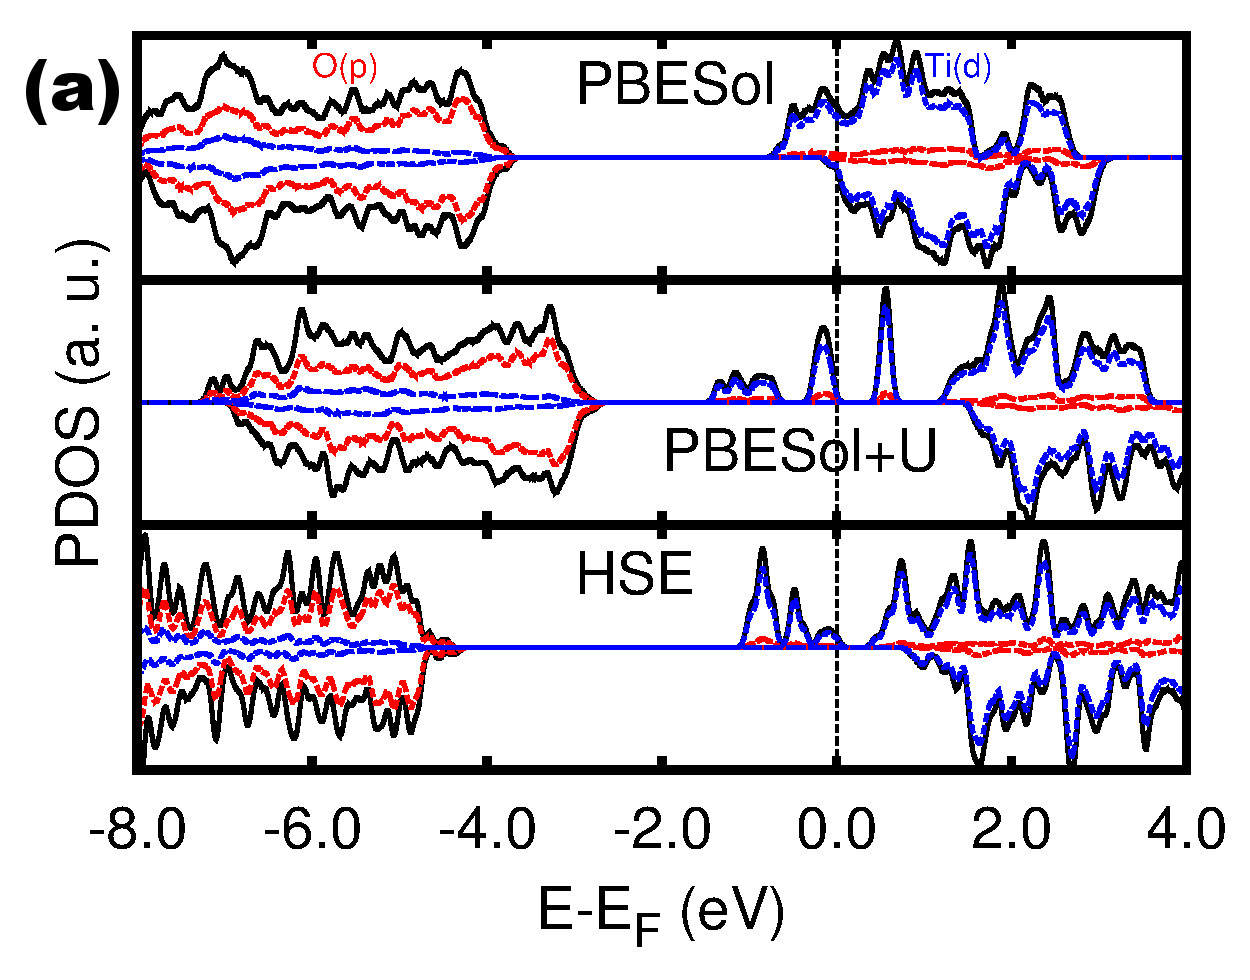
\includegraphics[width=0.3\textwidth]{img/dos-alpha-ti3o5.jpg}
        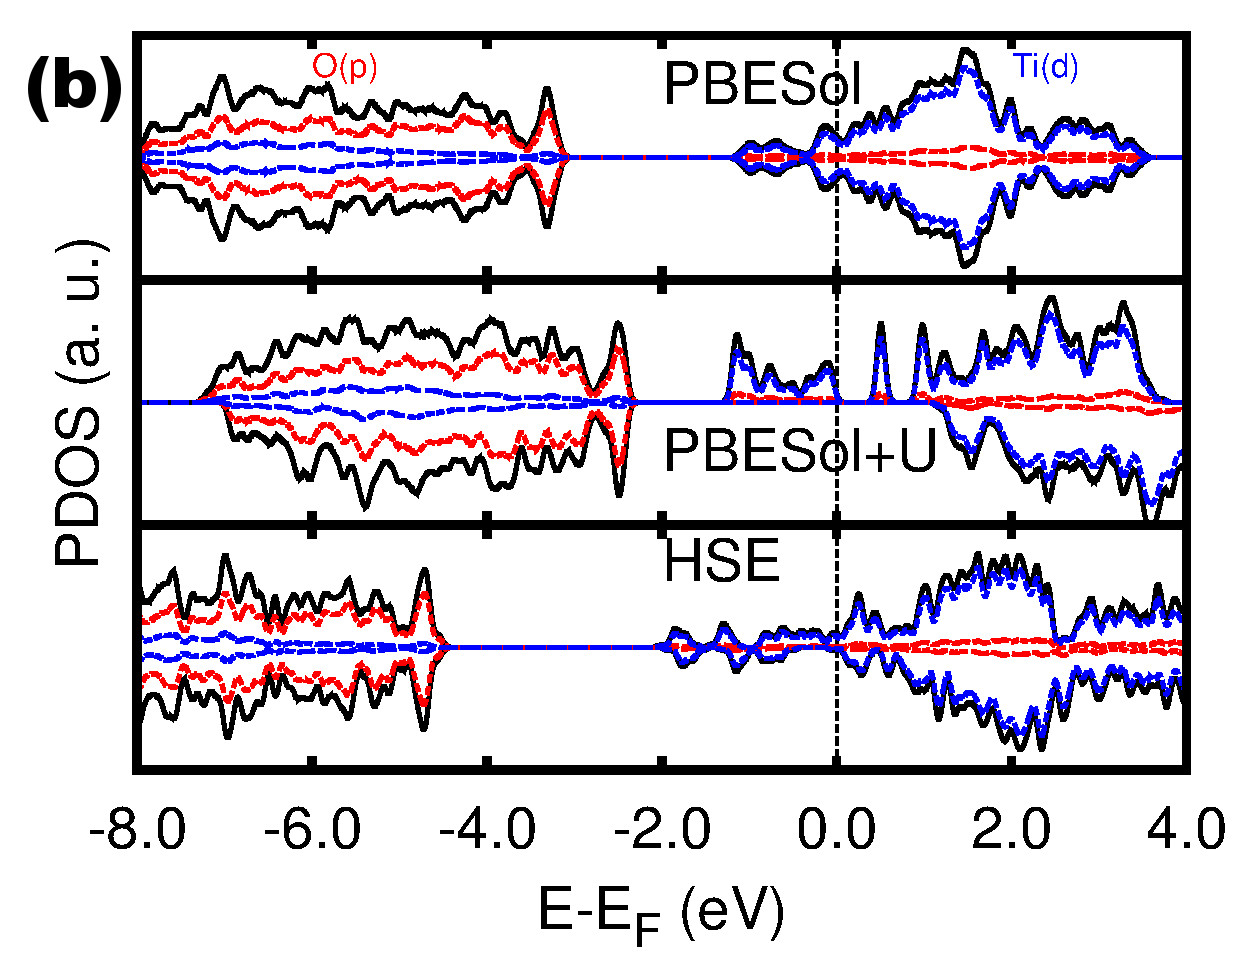
\includegraphics[width=0.3\textwidth]{img/dos-beta-ti3o5.jpg}
        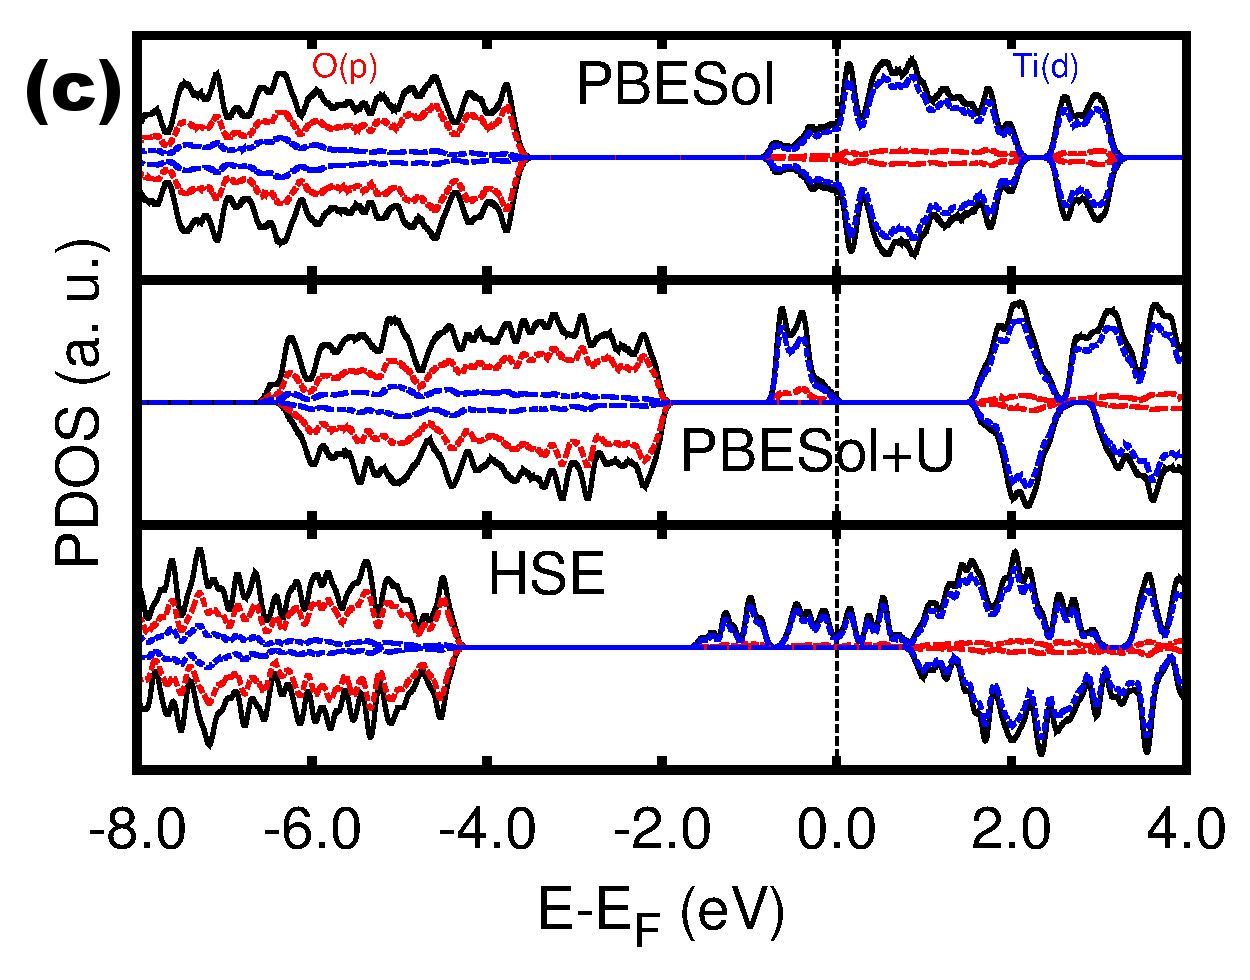
\includegraphics[width=0.3\textwidth]{img/dos-gamma-ti3o5.jpg} 
      \end{center}
      \caption{PDOS of (a) $\alpha$-Ti$_3$O$_5$, (b) $\beta$-Ti$_3$O$_5$, and (c) $\gamma$-Ti$_3$O$_5$ calculated by PBESol (upper panel), PBESol$+U$, where $U = 5$ eV (middle panel), and HSE (lower panel). The two spin components are depicted by positive and negative values along the vertical axis, and the vertical dashed line features the most energetic occupied level. The contribution from Ti(d) to CB and O(p) to VB are depicted by the blue and red dashed lines respectively while total DOS is given by the black full line.}.
      \label{fig:dos-ti3o5-prb} 
  \end{figure}
\end{center}

\section{Ti$_4$O$_7$ and Ti$_5$O$_9$ Magnéli phases}
\label{sec:magneli}

The results reported in this section, for both Ti$_4$O$_7$ and Ti$_5$O$_9$ Magnéli phases are the most important among those oxygen-deficient compounds, due to the fact that channels composed of these structures were detected inside memristors (see figure \ref{fig:canais-TiO}). 
\begin{figure}[!ht]
\centering
  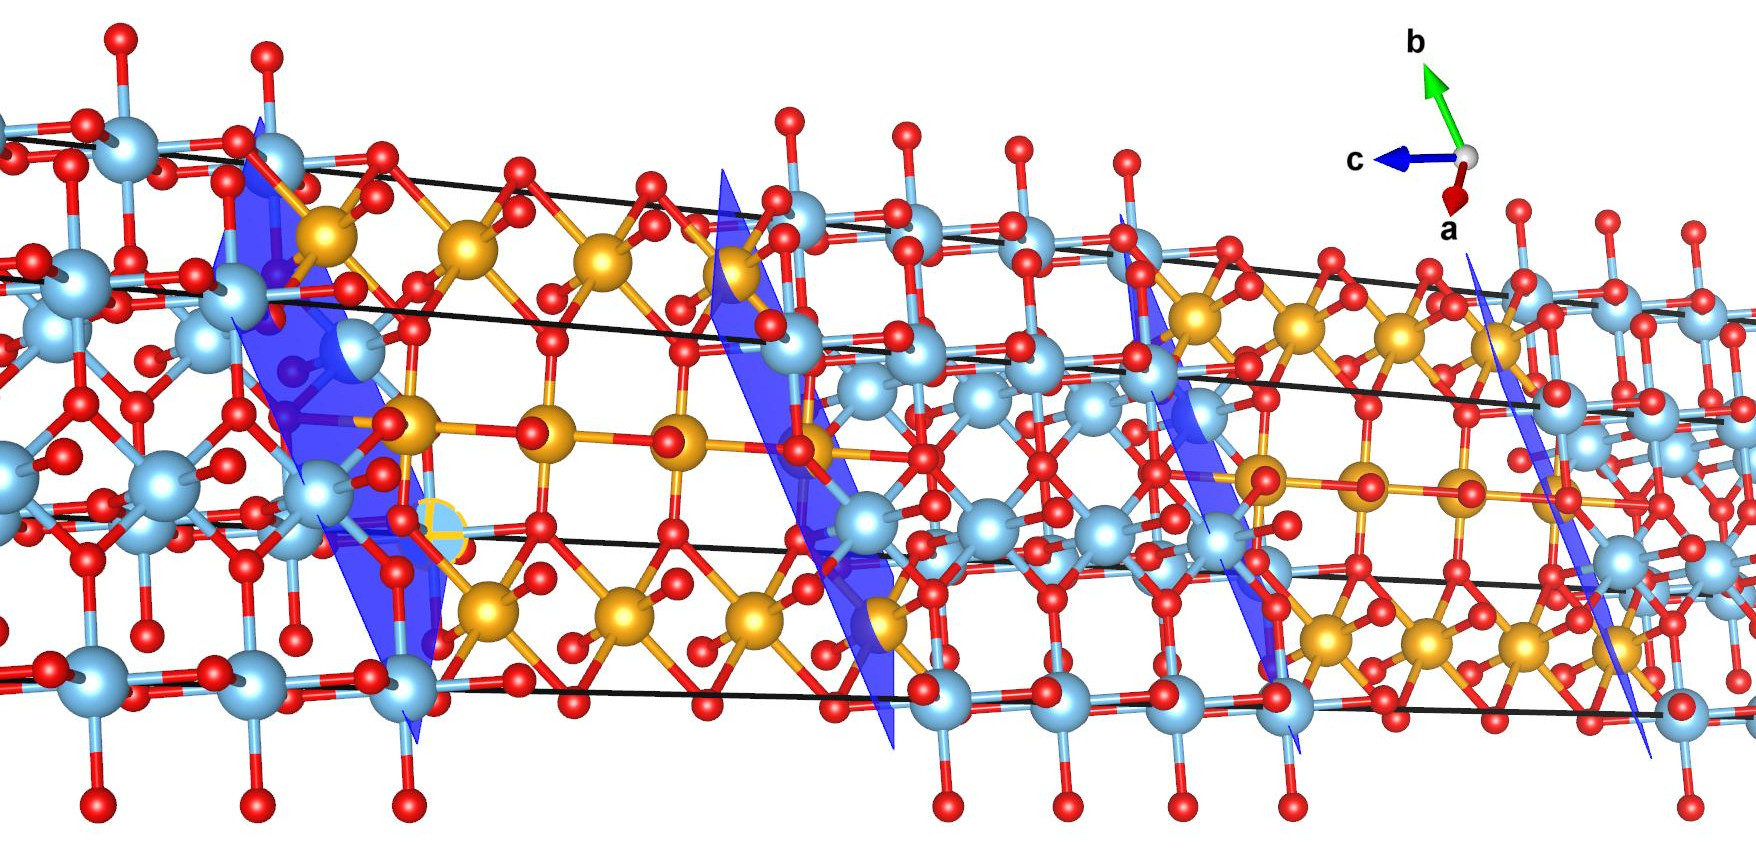
\includegraphics[width=0.9\textwidth]{img/ti4o7-multiple-c.jpg}
  \caption{Crystalline structure of Ti$_4$O$_7$. The blue and golden spheres are Ti atoms while the red spheres are O atoms. Different colors were used for Ti atoms to emphasize the rutile-like chains bounded by the shear planes, which are on the $ab$-plane and are featured in blue.}% The inset shows a cut of the same structure where the rutile-like chains are contained in the plane of the page. Ti$_5$O$_9$ presents a similar structure with one TiO$_6$ octahedra longer rutile-like chains.} 
  \label{fig:ti4o7-struct}
\end{figure}

All Magnéli phases are also composed of TiO$_6$ octahedra and present general formula Ti$_n$O$_{2n-1}$ ($4 \leq n \leq 10$), where $n$ is the number of octahedra in a rutile-like chain bounded by corundum-like structures. An illustration of the Ti$_4$O$_7$ structure is presented in figure \ref{fig:ti4o7-struct}. Ti$_4$O$_7$ presents three phases: low-temperature (LT, $T \leq$ 140 K), intermediate-temperature (IT, 140 K $\leq T \leq$ 150 K), and high temperature (HT, $T >$ 150 K) \cite{Bartholomew1969}. All phases present triclinic unit cell and space group $P\bar{1}$ \cite{LePage1984,Marezio1973,Marezio1971}, being the only difference between the structures a slight displacement of the atoms with respect to each other. After ionic relaxation, all structures converged to the same energy minimum with respect to ionic coordinates, thus, we report only the calculations for the LT phase. Ti$_5$O$_9$ has also a triclinic cell and space group $P1$ \cite{Andersson1960}.

The methodology employed for the previous materials was again tested for Ti$_4$O$_7$ calculations, and the band structure of this material is presented for LDA$+U$ functional [$0 \leq U \leq 5$ eV for Ti(d) electrons] in figure \ref{fig:bands-ti4o7}. The same behavior as in the Ti$_2$O$_3$ case was noticed: four bands became split from the unoccupied bands and a small gap of about 0.5 eV was observed when $U = 5$ eV.
\begin{figure}[!ht]
\centering
  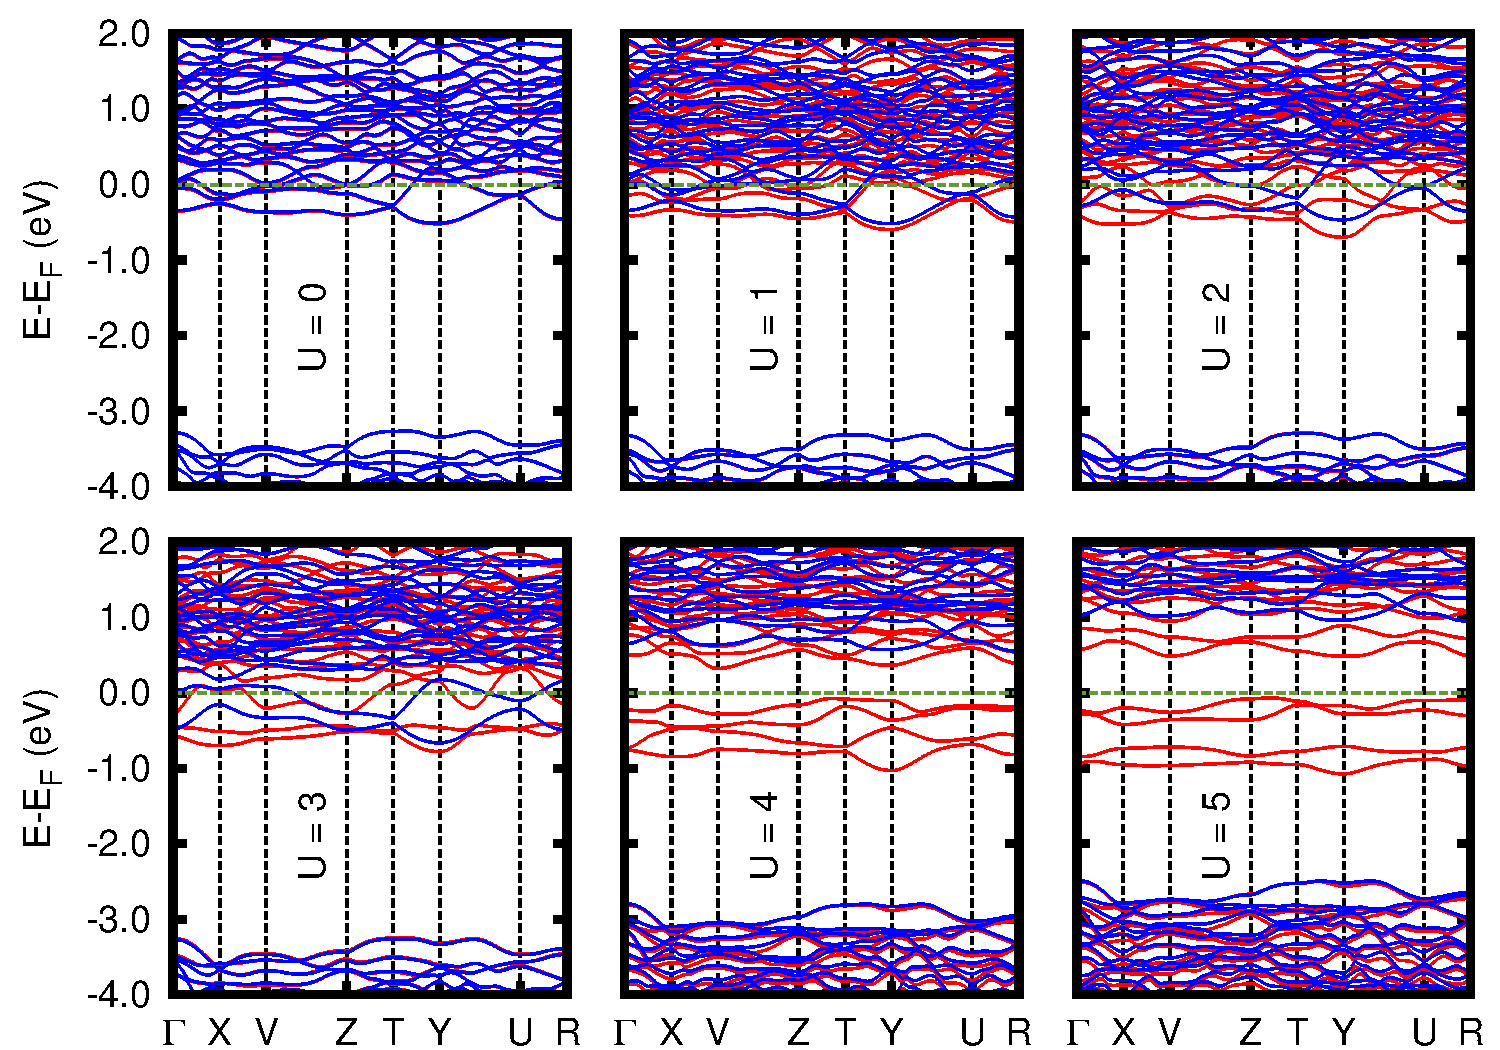
\includegraphics[width=0.95\textwidth]{img/bands-ti4o7.jpg}
  \caption{Band structure of Ti$_4$O$_7$ obtained using LDA+$U$ for increasing values of the Hubbard parameter $U$, ($0 \leq U \leq 5$). The spin components are plotted using either blue or red curves and the vertical green dashed line at zero energy is the Fermi energy. For $U = 4$ and $5$ the system is a semiconductor, while in the other cases it is a metal.} 
  \label{fig:bands-ti4o7}
\end{figure}

Comparison with PBESol, PBESol$+U$, and HSE functionals was made by plotting the PDOS of those systems. The results for both Ti$_4$O$_7$ and Ti$_5$O$_9$ are presented in figure \ref{fig:dos-magneli-prb}. From those graphs it is possible to notice that PBESol describes both systems as metals while the use of $U$ for Ti(d) electrons or HSE functional describe Ti$_4$O$_7$ and Ti$_5$O$_9$ as a small gap and large gap semiconductors respectively. The description of the electronic structure in these cases can be analogous to the previous discussion for Ti$_2$O$_3$: CB is mainly of Ti(d) contribution, VB is O(p), and IB has Ti(d) character. Comparison with experimental data in this case is difficult once there are no reports of the bandgap energy for Ti$_5$O$_9$, and for Ti$_4$O$_7$ a handful of values, from nearly metallic (0.041 eV from conductivity measurements \cite{Mulay1970}) to small-gap semiconductor (0.6 eV from spectroscopy analysis \cite{Abbate1995}), was reported.
\begin{center}
  \begin{figure}[ht!]
      \begin{center}
        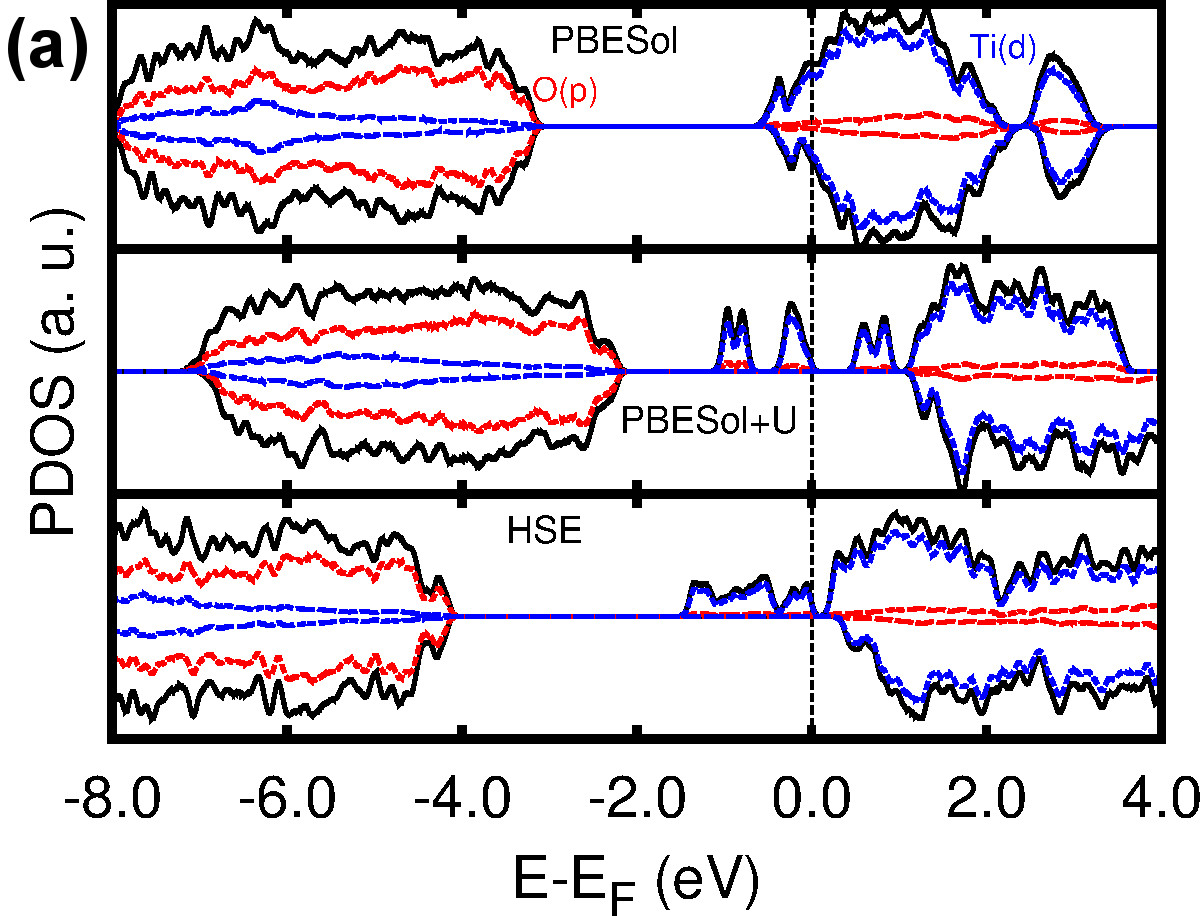
\includegraphics[width=0.45\textwidth]{img/dos-ti4o7-prb.jpg}
        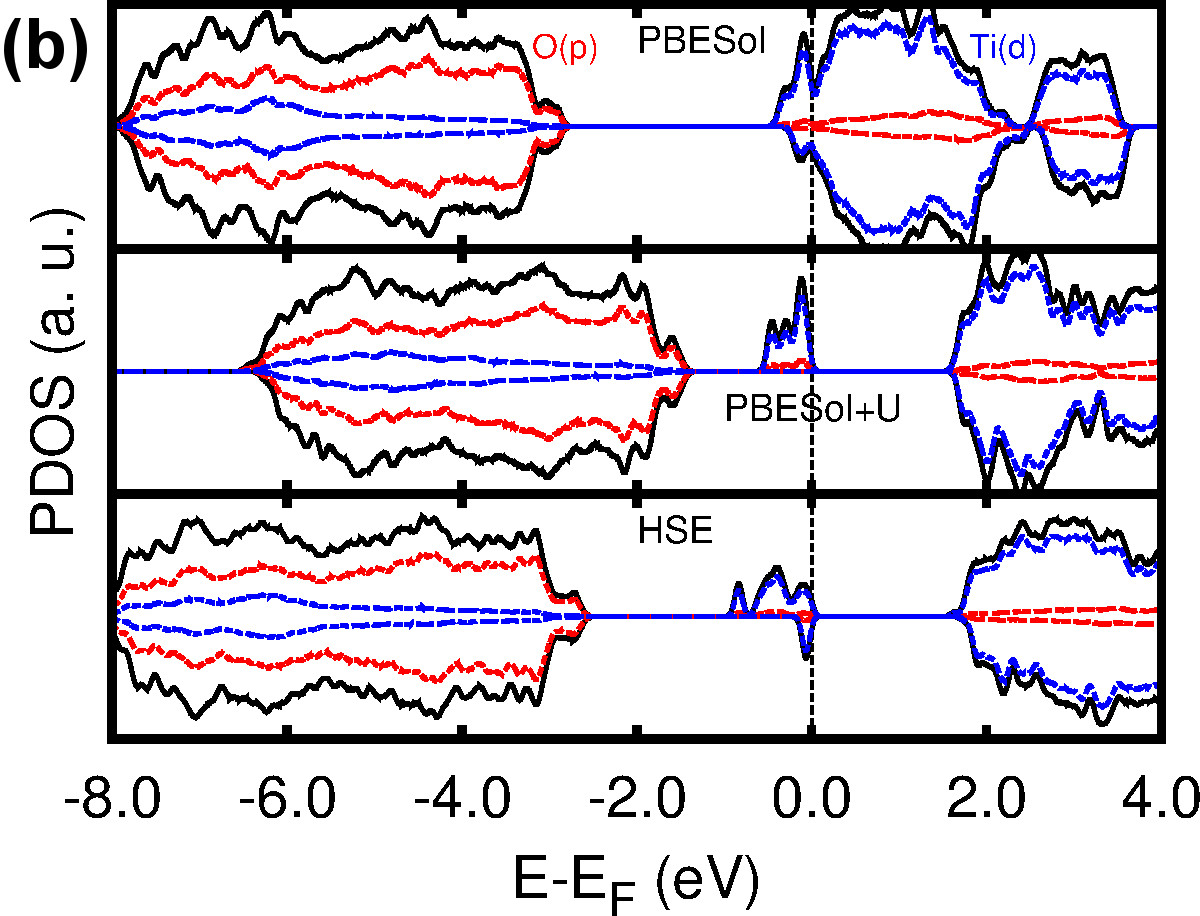
\includegraphics[width=0.45\textwidth]{img/dos-ti5o9-prb.jpg} 
      \end{center}
      \caption{PDOS of (a) Ti$_4$O$_7$, and (b) Ti$_5$O$_9$ calculated by PBESol (upper panel), PBESol$+U$, where $U = 5$ eV (middle panel), and HSE (lower panel). The two spin components are depicted by positive and negative values along the vertical axis, and the vertical dashed line features the most energetic occupied level. The contribution from Ti(d) to CB and O(p) to VB are depicted by the blue and red dashed lines respectively while total DOS is given by the black full line.}.
      \label{fig:dos-magneli-prb} 
  \end{figure}
\end{center}

Real-space projection of the IB of Ti$_4$O$_7$ was obtained in the same way as it was done for Ti$_2$O$_3$. The visual inspection of the orbitals plotted in figure \ref{fig:ti4o7-parchg} reveals a better localization by both PBESol$+U$ and HSE in comparison with PBESol calculation.
\begin{center}
  \begin{figure}[ht!]
      \begin{center}
        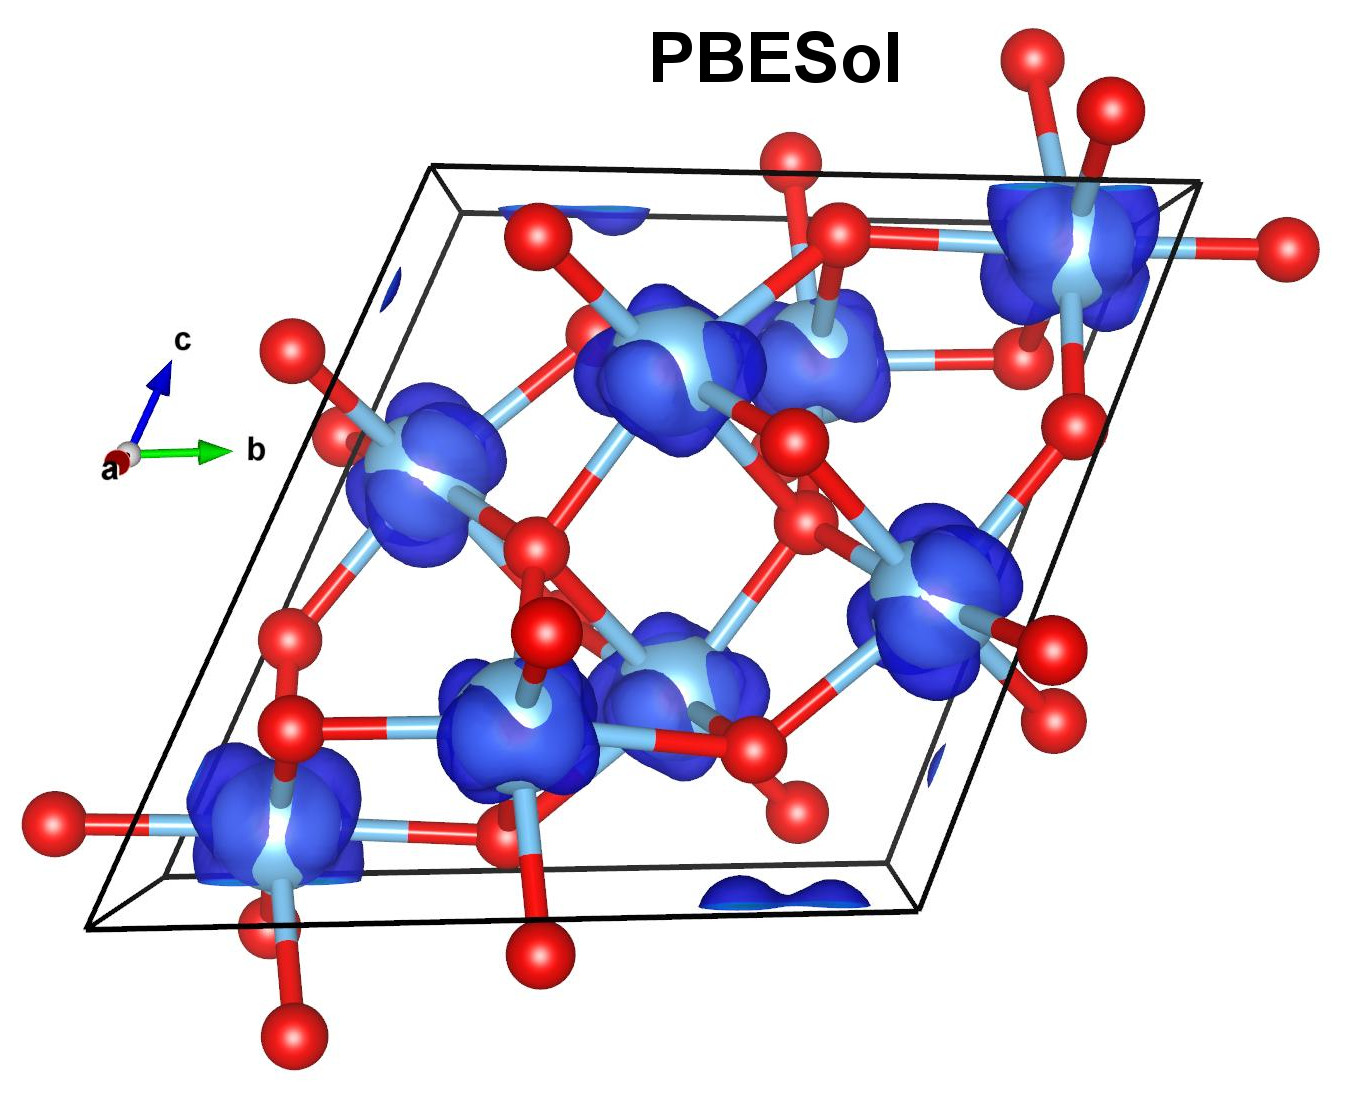
\includegraphics[width=0.3\textwidth]{img/ti4o7-parchg-pbsol+u0.jpg}
        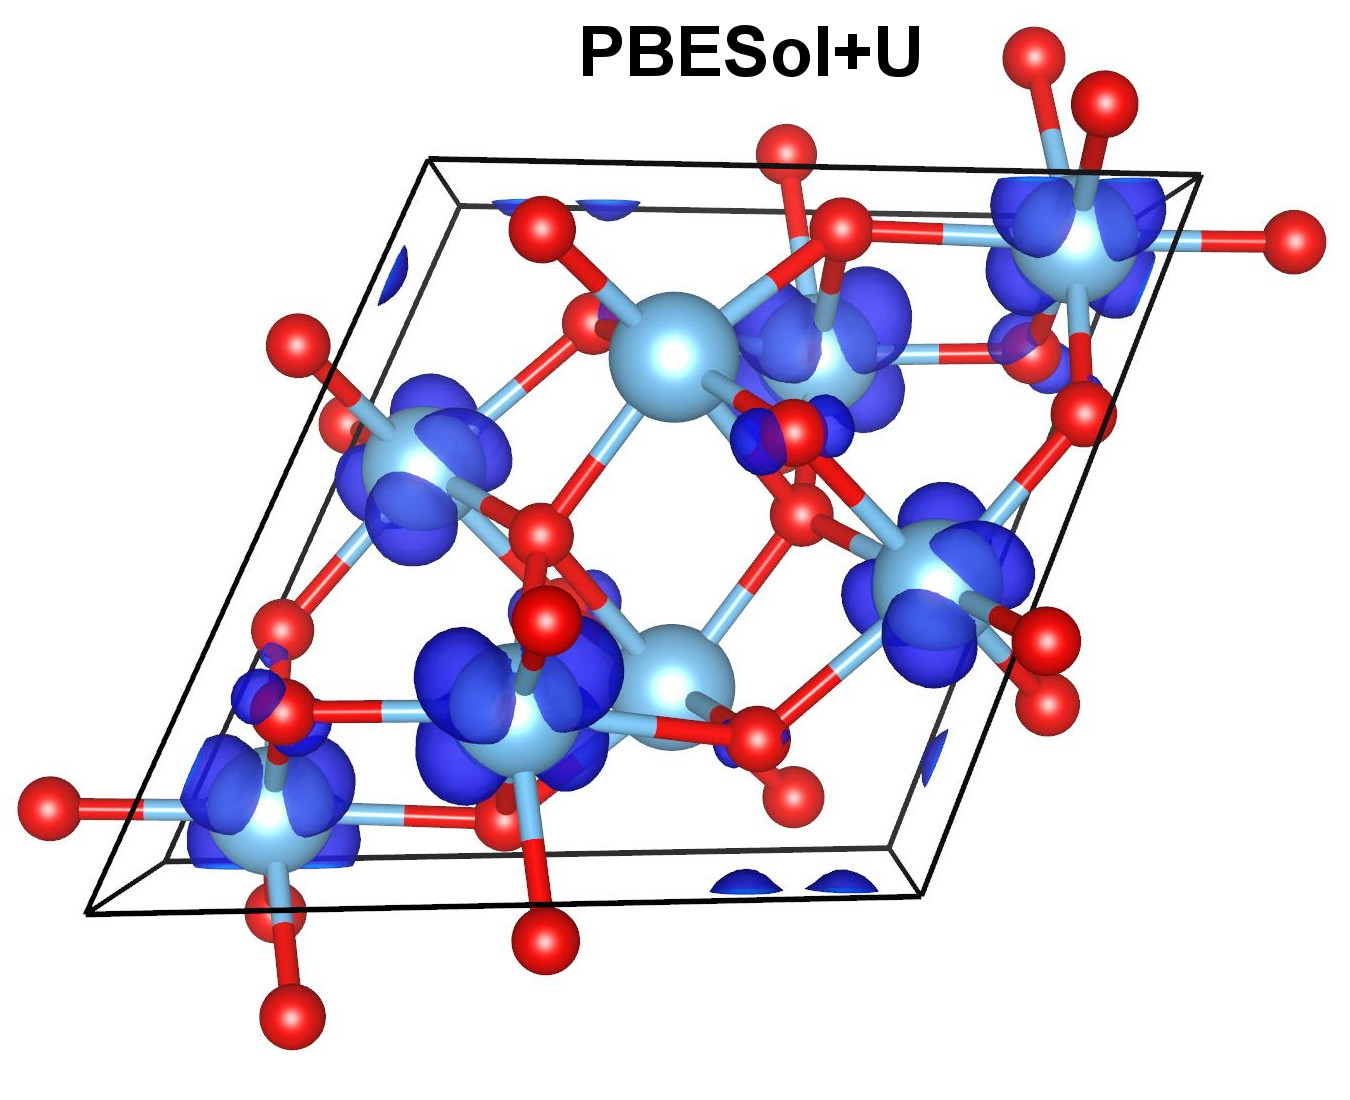
\includegraphics[width=0.3\textwidth]{img/ti4o7-parchg-pbsol+u5.jpg}
        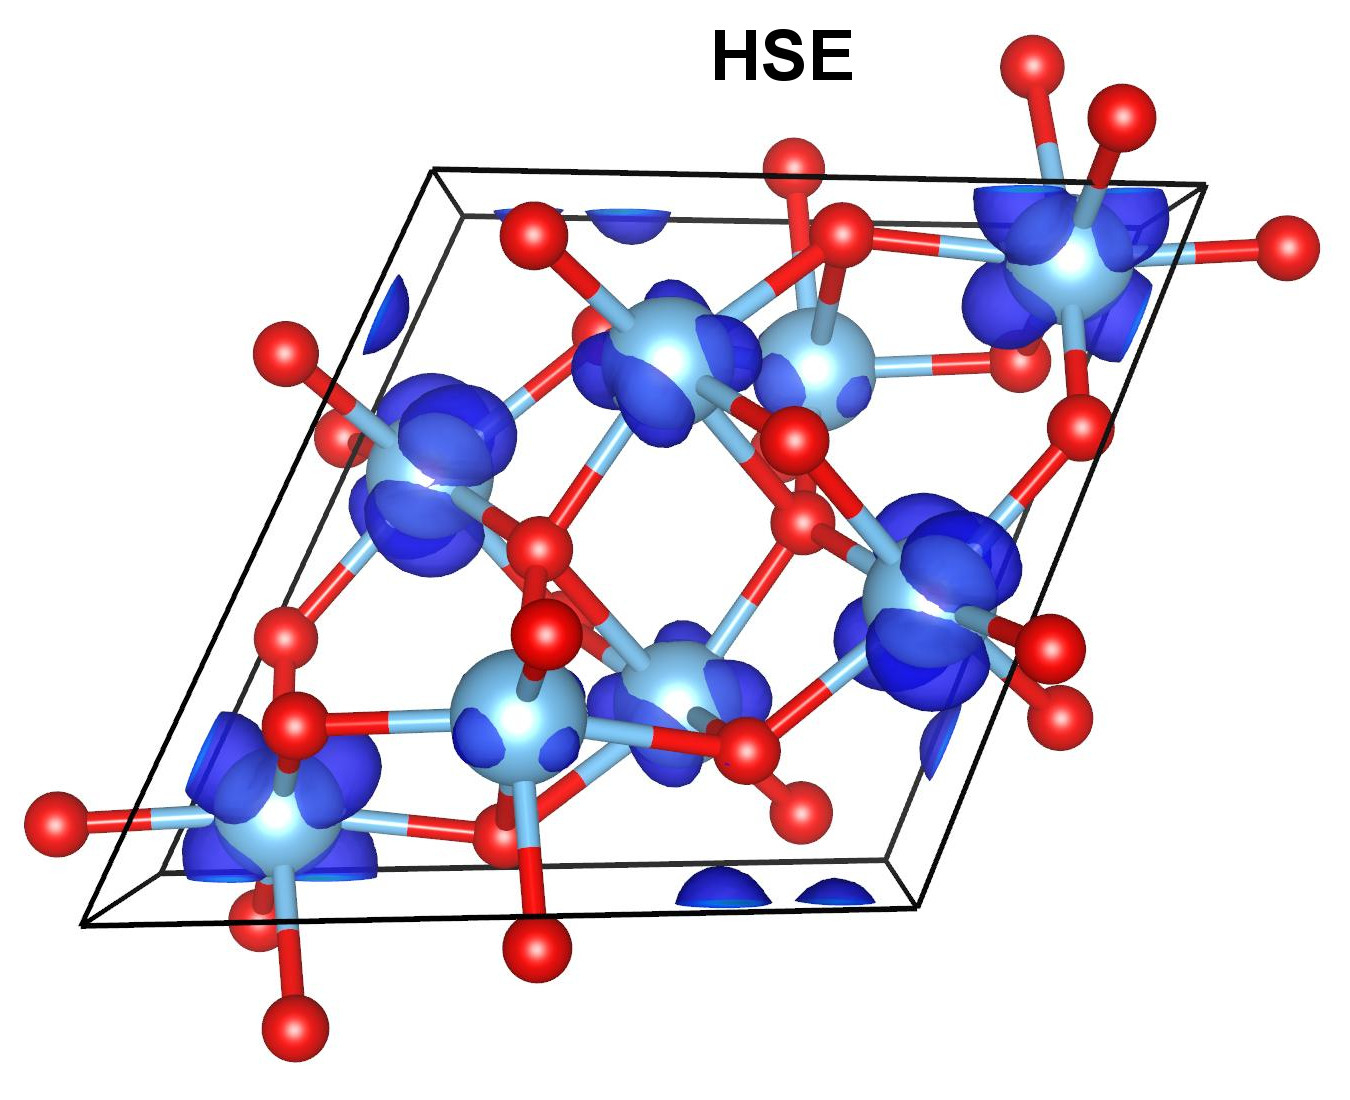
\includegraphics[width=0.3\textwidth]{img/ti4o7-parchg-hse.jpg}
      \end{center}
      \caption{Real-space projection over the primitive cell of the IB of Ti$_4$O$_7$ calculated by PBESol (left), PBESol$+U$, where $U = 5$ eV (middle), and HSE (right). The same isovalue of 1\% was used to plot the three bands.}.
      \label{fig:ti4o7-parchg} 
  \end{figure}
\end{center}

\section{Oxygen-deficiency in TiO$_2$}

Whenever native point defects are introduced into TiO$_2$, an excess of electron arises due to the deviation from stoichiometry. In the case of oxygen vacancy introduction (\textit{i. e.} the removal o oxygen atoms), a pair of unbound electrons is left behind, and if titanium interstitials are inserted, due to the $3d^24s^2$ configuration, a similar situation takes place \cite{Janotti2010,Lee2012}. With the exception of Ti$_2$O$_3$, which is a diamagnet at low temperatures \cite{Guo2012}, all the other oxygen-deficient phases of TiO$_2$ might present some degree of magnetism. Table \ref{tab:mags} shows the resulting total magnetization density per unit cell [$\mu(\mathrm{r})=\rho_{\uparrow}(\mathrm{r})-\rho_{\downarrow}(\mathrm{r})$] for all those systems. There it is noticeable that, with exception of $\beta$-Ti$_3$O$_5$ and Ti$_5$O$_9$, the magnetization density results for both PBESol$+U$ and HSE are essentially the same, indicating the presence of four parallel-spin electrons per cell\footnote{The unit cells of all systems presented here comprise two formula units, thus, the expected number in this case is indeed 4 $\mu_B$.}. This is an evidence of the better suitability of these methods rather than pure GGA functionals to study these crystals, and additionally, the PBESol$+U$ leads to even better results in comparison to HSE. This might be due to the fact that the energy landscape with respect to spin polarization degree of freedom presents a series of local minima, being necessary a more computationally expensive method to fully map the possible configurations of minimum energy, as \textit{e. g.} quantum dynamics or annealing methods.
\begin{table}[ht!]
  \centering
  \caption{\label{tab:mags} Total magnetization per unit cell in units of Bohr magnetons ($\mu_B$) for all Ti${}_n$O${}_{2n-1}$ structures presented in this work obtained with PBESol, PBESol$+U$, and HSE functionals.}
   \begin{tabular}{*{7}{c}}
  \hhline{=======} 
    & Ti${}_2$O${}_3$ & $\alpha$-Ti${}_3$O${}_5$ & $\beta$-Ti$_3$O$_5$ & $\gamma$-Ti$_3$O$_5$ & Ti${}_4$O${}_7$ & Ti${}_5$O${}_9$ \\
    \hline
   PBESol & -0.06  & 3.75   & 0.00    & 0.15    & 1.12       & 2.19                    \\
    %\hline
     PBESol$+U$ &  0.00    & 4.00   & 3.99     & 4.00   & 4.00       & 4.00           \\
    %\hline
  HSE &  0.00   & 4.00   & 0.94  & 4.00   & 4.00     & 2.75      \\ 
  \hhline{=======} 
   \end{tabular}
 \end{table}

As a final remark, these results point towards the existence of an \textit{intermediate band} inside the bandgap for all the oxygen-deficient phases of TiO$_2$. These levels are close to the conduction band in all cases, and their character is mainly of Ti(d). This is similar to what is reported about point defects in the TiO$_2$ \cite{Janotti2010,Lee2012}. Owing to the fact that the Fermi level lies above those levels, charge transfer from them to the unoccupied levels can take place if an external perturbation is introduced in the system, as an external voltage---this is exactly what happens in the operation of a memristor. 

Indeed, some of those systems were already studied by DFT calculations: Guo \textit{et al.} used a screened exact exchange functional and reported an indirect ($L-\Gamma$) bandgap of 0.55 eV for Ti$_2$O$_3$ in agreement with our calculations \cite{Guo2012}. The three phases of Ti$_4$O$_7$ were studied by Liborio \textit{et al.} using B3LYP hybrid functional, resulting in small gaps and electronic levels similar to our IB \cite{Liborio2009}, while Weissmann reported HT-Ti$_4$O$_7$ as a metal and both IT- and LT-Ti$_4$O$_7$ as semiconductors using LDA+$U$ level of theory \cite{Weissmann2011}. Leonov reported a bandgap of 0.29 eV using the same methods \cite{Leonov2006}. Slipukhina and Le\v{z}ai\'{c} reported a very similar behavior to what is reported in this chapter with respect to increasing values of the $U$ parameter \cite{Slipukhina2014}. Our results present a systematic comparison between methodologies, by using both the GGA functional PBESol without and with the Hubbard $U$, and the hybrid functional HSE, showing that are compatible with these previous reports, as well as with the experimental data on the electrical properties of these systems. In this sense, our contribution in the study of these oxygen-deficient phases is a step further in the literature, by showing that these methods are suitable for further, more intrincate studies on these materials, being the use of the Hubbard $U$ a faster a reliable way in comparison with hybrids. The majority of the results presented in this chapter were published in Physical Review B \cite{Padilha2014}. The article is attached to this thesis in appendix \ref{sec:app-pub}.